% Options for packages loaded elsewhere
\PassOptionsToPackage{unicode}{hyperref}
\PassOptionsToPackage{hyphens}{url}
\PassOptionsToPackage{dvipsnames,svgnames,x11names}{xcolor}
%
\documentclass[
  letterpaper,
  DIV=11,
  numbers=noendperiod]{scrreprt}

\usepackage{amsmath,amssymb}
\usepackage{iftex}
\ifPDFTeX
  \usepackage[T1]{fontenc}
  \usepackage[utf8]{inputenc}
  \usepackage{textcomp} % provide euro and other symbols
\else % if luatex or xetex
  \usepackage{unicode-math}
  \defaultfontfeatures{Scale=MatchLowercase}
  \defaultfontfeatures[\rmfamily]{Ligatures=TeX,Scale=1}
\fi
\usepackage{lmodern}
\ifPDFTeX\else  
    % xetex/luatex font selection
\fi
% Use upquote if available, for straight quotes in verbatim environments
\IfFileExists{upquote.sty}{\usepackage{upquote}}{}
\IfFileExists{microtype.sty}{% use microtype if available
  \usepackage[]{microtype}
  \UseMicrotypeSet[protrusion]{basicmath} % disable protrusion for tt fonts
}{}
\makeatletter
\@ifundefined{KOMAClassName}{% if non-KOMA class
  \IfFileExists{parskip.sty}{%
    \usepackage{parskip}
  }{% else
    \setlength{\parindent}{0pt}
    \setlength{\parskip}{6pt plus 2pt minus 1pt}}
}{% if KOMA class
  \KOMAoptions{parskip=half}}
\makeatother
\usepackage{xcolor}
\setlength{\emergencystretch}{3em} % prevent overfull lines
\setcounter{secnumdepth}{5}
% Make \paragraph and \subparagraph free-standing
\ifx\paragraph\undefined\else
  \let\oldparagraph\paragraph
  \renewcommand{\paragraph}[1]{\oldparagraph{#1}\mbox{}}
\fi
\ifx\subparagraph\undefined\else
  \let\oldsubparagraph\subparagraph
  \renewcommand{\subparagraph}[1]{\oldsubparagraph{#1}\mbox{}}
\fi

\usepackage{color}
\usepackage{fancyvrb}
\newcommand{\VerbBar}{|}
\newcommand{\VERB}{\Verb[commandchars=\\\{\}]}
\DefineVerbatimEnvironment{Highlighting}{Verbatim}{commandchars=\\\{\}}
% Add ',fontsize=\small' for more characters per line
\usepackage{framed}
\definecolor{shadecolor}{RGB}{241,243,245}
\newenvironment{Shaded}{\begin{snugshade}}{\end{snugshade}}
\newcommand{\AlertTok}[1]{\textcolor[rgb]{0.68,0.00,0.00}{#1}}
\newcommand{\AnnotationTok}[1]{\textcolor[rgb]{0.37,0.37,0.37}{#1}}
\newcommand{\AttributeTok}[1]{\textcolor[rgb]{0.40,0.45,0.13}{#1}}
\newcommand{\BaseNTok}[1]{\textcolor[rgb]{0.68,0.00,0.00}{#1}}
\newcommand{\BuiltInTok}[1]{\textcolor[rgb]{0.00,0.23,0.31}{#1}}
\newcommand{\CharTok}[1]{\textcolor[rgb]{0.13,0.47,0.30}{#1}}
\newcommand{\CommentTok}[1]{\textcolor[rgb]{0.37,0.37,0.37}{#1}}
\newcommand{\CommentVarTok}[1]{\textcolor[rgb]{0.37,0.37,0.37}{\textit{#1}}}
\newcommand{\ConstantTok}[1]{\textcolor[rgb]{0.56,0.35,0.01}{#1}}
\newcommand{\ControlFlowTok}[1]{\textcolor[rgb]{0.00,0.23,0.31}{#1}}
\newcommand{\DataTypeTok}[1]{\textcolor[rgb]{0.68,0.00,0.00}{#1}}
\newcommand{\DecValTok}[1]{\textcolor[rgb]{0.68,0.00,0.00}{#1}}
\newcommand{\DocumentationTok}[1]{\textcolor[rgb]{0.37,0.37,0.37}{\textit{#1}}}
\newcommand{\ErrorTok}[1]{\textcolor[rgb]{0.68,0.00,0.00}{#1}}
\newcommand{\ExtensionTok}[1]{\textcolor[rgb]{0.00,0.23,0.31}{#1}}
\newcommand{\FloatTok}[1]{\textcolor[rgb]{0.68,0.00,0.00}{#1}}
\newcommand{\FunctionTok}[1]{\textcolor[rgb]{0.28,0.35,0.67}{#1}}
\newcommand{\ImportTok}[1]{\textcolor[rgb]{0.00,0.46,0.62}{#1}}
\newcommand{\InformationTok}[1]{\textcolor[rgb]{0.37,0.37,0.37}{#1}}
\newcommand{\KeywordTok}[1]{\textcolor[rgb]{0.00,0.23,0.31}{#1}}
\newcommand{\NormalTok}[1]{\textcolor[rgb]{0.00,0.23,0.31}{#1}}
\newcommand{\OperatorTok}[1]{\textcolor[rgb]{0.37,0.37,0.37}{#1}}
\newcommand{\OtherTok}[1]{\textcolor[rgb]{0.00,0.23,0.31}{#1}}
\newcommand{\PreprocessorTok}[1]{\textcolor[rgb]{0.68,0.00,0.00}{#1}}
\newcommand{\RegionMarkerTok}[1]{\textcolor[rgb]{0.00,0.23,0.31}{#1}}
\newcommand{\SpecialCharTok}[1]{\textcolor[rgb]{0.37,0.37,0.37}{#1}}
\newcommand{\SpecialStringTok}[1]{\textcolor[rgb]{0.13,0.47,0.30}{#1}}
\newcommand{\StringTok}[1]{\textcolor[rgb]{0.13,0.47,0.30}{#1}}
\newcommand{\VariableTok}[1]{\textcolor[rgb]{0.07,0.07,0.07}{#1}}
\newcommand{\VerbatimStringTok}[1]{\textcolor[rgb]{0.13,0.47,0.30}{#1}}
\newcommand{\WarningTok}[1]{\textcolor[rgb]{0.37,0.37,0.37}{\textit{#1}}}

\providecommand{\tightlist}{%
  \setlength{\itemsep}{0pt}\setlength{\parskip}{0pt}}\usepackage{longtable,booktabs,array}
\usepackage{calc} % for calculating minipage widths
% Correct order of tables after \paragraph or \subparagraph
\usepackage{etoolbox}
\makeatletter
\patchcmd\longtable{\par}{\if@noskipsec\mbox{}\fi\par}{}{}
\makeatother
% Allow footnotes in longtable head/foot
\IfFileExists{footnotehyper.sty}{\usepackage{footnotehyper}}{\usepackage{footnote}}
\makesavenoteenv{longtable}
\usepackage{graphicx}
\makeatletter
\def\maxwidth{\ifdim\Gin@nat@width>\linewidth\linewidth\else\Gin@nat@width\fi}
\def\maxheight{\ifdim\Gin@nat@height>\textheight\textheight\else\Gin@nat@height\fi}
\makeatother
% Scale images if necessary, so that they will not overflow the page
% margins by default, and it is still possible to overwrite the defaults
% using explicit options in \includegraphics[width, height, ...]{}
\setkeys{Gin}{width=\maxwidth,height=\maxheight,keepaspectratio}
% Set default figure placement to htbp
\makeatletter
\def\fps@figure{htbp}
\makeatother
% definitions for citeproc citations
\NewDocumentCommand\citeproctext{}{}
\NewDocumentCommand\citeproc{mm}{%
  \begingroup\def\citeproctext{#2}\cite{#1}\endgroup}
\makeatletter
 % allow citations to break across lines
 \let\@cite@ofmt\@firstofone
 % avoid brackets around text for \cite:
 \def\@biblabel#1{}
 \def\@cite#1#2{{#1\if@tempswa , #2\fi}}
\makeatother
\newlength{\cslhangindent}
\setlength{\cslhangindent}{1.5em}
\newlength{\csllabelwidth}
\setlength{\csllabelwidth}{3em}
\newenvironment{CSLReferences}[2] % #1 hanging-indent, #2 entry-spacing
 {\begin{list}{}{%
  \setlength{\itemindent}{0pt}
  \setlength{\leftmargin}{0pt}
  \setlength{\parsep}{0pt}
  % turn on hanging indent if param 1 is 1
  \ifodd #1
   \setlength{\leftmargin}{\cslhangindent}
   \setlength{\itemindent}{-1\cslhangindent}
  \fi
  % set entry spacing
  \setlength{\itemsep}{#2\baselineskip}}}
 {\end{list}}
\usepackage{calc}
\newcommand{\CSLBlock}[1]{\hfill\break\parbox[t]{\linewidth}{\strut\ignorespaces#1\strut}}
\newcommand{\CSLLeftMargin}[1]{\parbox[t]{\csllabelwidth}{\strut#1\strut}}
\newcommand{\CSLRightInline}[1]{\parbox[t]{\linewidth - \csllabelwidth}{\strut#1\strut}}
\newcommand{\CSLIndent}[1]{\hspace{\cslhangindent}#1}

\KOMAoption{captions}{tableheading}
\makeatletter
\@ifpackageloaded{tcolorbox}{}{\usepackage[skins,breakable]{tcolorbox}}
\@ifpackageloaded{fontawesome5}{}{\usepackage{fontawesome5}}
\definecolor{quarto-callout-color}{HTML}{909090}
\definecolor{quarto-callout-note-color}{HTML}{0758E5}
\definecolor{quarto-callout-important-color}{HTML}{CC1914}
\definecolor{quarto-callout-warning-color}{HTML}{EB9113}
\definecolor{quarto-callout-tip-color}{HTML}{00A047}
\definecolor{quarto-callout-caution-color}{HTML}{FC5300}
\definecolor{quarto-callout-color-frame}{HTML}{acacac}
\definecolor{quarto-callout-note-color-frame}{HTML}{4582ec}
\definecolor{quarto-callout-important-color-frame}{HTML}{d9534f}
\definecolor{quarto-callout-warning-color-frame}{HTML}{f0ad4e}
\definecolor{quarto-callout-tip-color-frame}{HTML}{02b875}
\definecolor{quarto-callout-caution-color-frame}{HTML}{fd7e14}
\makeatother
\makeatletter
\@ifpackageloaded{bookmark}{}{\usepackage{bookmark}}
\makeatother
\makeatletter
\@ifpackageloaded{caption}{}{\usepackage{caption}}
\AtBeginDocument{%
\ifdefined\contentsname
  \renewcommand*\contentsname{Table of contents}
\else
  \newcommand\contentsname{Table of contents}
\fi
\ifdefined\listfigurename
  \renewcommand*\listfigurename{List of Figures}
\else
  \newcommand\listfigurename{List of Figures}
\fi
\ifdefined\listtablename
  \renewcommand*\listtablename{List of Tables}
\else
  \newcommand\listtablename{List of Tables}
\fi
\ifdefined\figurename
  \renewcommand*\figurename{Figure}
\else
  \newcommand\figurename{Figure}
\fi
\ifdefined\tablename
  \renewcommand*\tablename{Table}
\else
  \newcommand\tablename{Table}
\fi
}
\@ifpackageloaded{float}{}{\usepackage{float}}
\floatstyle{ruled}
\@ifundefined{c@chapter}{\newfloat{codelisting}{h}{lop}}{\newfloat{codelisting}{h}{lop}[chapter]}
\floatname{codelisting}{Listing}
\newcommand*\listoflistings{\listof{codelisting}{List of Listings}}
\makeatother
\makeatletter
\makeatother
\makeatletter
\@ifpackageloaded{caption}{}{\usepackage{caption}}
\@ifpackageloaded{subcaption}{}{\usepackage{subcaption}}
\makeatother
\ifLuaTeX
  \usepackage{selnolig}  % disable illegal ligatures
\fi
\usepackage{bookmark}

\IfFileExists{xurl.sty}{\usepackage{xurl}}{} % add URL line breaks if available
\urlstyle{same} % disable monospaced font for URLs
\hypersetup{
  pdftitle={Data Science at SHARE Creative},
  pdfauthor={Jamie Hudson},
  colorlinks=true,
  linkcolor={blue},
  filecolor={Maroon},
  citecolor={Blue},
  urlcolor={Blue},
  pdfcreator={LaTeX via pandoc}}

\title{Data Science at SHARE Creative}
\author{Jamie Hudson}
\date{2024-05-07}

\begin{document}
\maketitle

\renewcommand*\contentsname{Table of contents}
{
\hypersetup{linkcolor=}
\setcounter{tocdepth}{2}
\tableofcontents
}
\bookmarksetup{startatroot}

\chapter*{Preface to handbook}\label{preface-to-handbook}
\addcontentsline{toc}{chapter}{Preface to handbook}

\markboth{Preface to handbook}{Preface to handbook}

This section will provide an overview of this handbook.

\subsection*{Handbook styling guide}\label{handbook-styling-guide}
\addcontentsline{toc}{subsection}{Handbook styling guide}

Timbo, we want this Handbook to appear written as a ``DS Scientist at
SHARE'' rather than the Jimbo + Timbo show. To help streamline this, I
suggest we follow the following guidelines to help ensure we are
consistent with our writing style. Some of these points will not be
relevant for all section, but I think we would be wise to always keep
them in the back of our mind throughout:

\begin{itemize}
\tightlist
\item
  Tone, we should be friendly but professional. We can definitely joke,
  but always try and make sure the point we are getting across is clear.
\item
  Let's make sure we use the active voice rather than passive voice and
  talk in the first person plural (i.e.~we, us rather than I, me etc).
\item
  If we are referring to a general data scientist or person, let's be
  inclusive and refer to them as ``they/them''. For example if we had
  the sentence ``Imagine a data scientist needs to embed a sentence,
  there are many models available on HuggingFace for \emph{them} to
  choose from''.
\item
  We need to take responsibility for what we write (this will be more
  relevant in the later sections of the handbook). We need to be make
  sure we understand concepts before committing them to the handbook-
  the creation of this handbook will not only help any newcomer get on
  board quicker, but also help cement DS concepts ourselves.
\end{itemize}

\begin{quote}
``If you can't explain it simply, you don't understand it well enough''
- Albert Einstein
\end{quote}

\bookmarksetup{startatroot}

\chapter{Glossary}\label{glossary}

\textbf{Embedding}: Numerical representations of real-world objects (in
the form of a vector of real numbers)

\textbf{Embedding Model}: A model that can perform embedding by
encapsulating information into dense representations in a
multi-dimensional space

\textbf{F1 Score}: The harmonic mean of precision and recall (enables us
to integrate precision and recall into a single metric)

\[
F1 \space Score = 2 \times \dfrac{Precision \times Recall}{Precision + Recall}
\]

\textbf{Precision}: The proportion of positive identifications that were
actually correct. Precision focuses on the correctness of positive
predictions

\[
Precision = \dfrac{TP}{(TP + FP) }
\]

\textbf{Recall}: The proportion of actual positives that were identified
correctly. Recall focuses on capturing all relevant instances

\[
Recall = \dfrac{TP}{(TP + FN) }
\]

\textbf{Sentence Embedding}: A numerical representation of a sentence

\textbf{Word Embedding}: A numerical representation of a single word

\bookmarksetup{startatroot}

\chapter{Peaks and Pits}\label{peaks-and-pits}

``Peak and Pits'' is one of our fundamental project offerings and a
workflow that is a solid representation of good data science work that
we perform.

\section{What is the concept/project
background?}\label{what-is-the-conceptproject-background}

Strong memories associated to brands or products go deeper than simple
positive or negative sentiment. Most of our experiences are not encoded
in memory, rather what we remember about experiences are changes,
significant moments, and endings. In their book ``The Power of
Moments'', two psychologists
(\href{https://heathbrothers.com/about/}{Chip and Dan Heath}) define
these core memories as Peak and Pits, impactful experiences in our
lives.

Broadly, peak moments are experiences that stand our memorable in our
lives in a positive sense, whereas pit moments are impactful negative
experiences.

Microsoft tasked us with finding a way to identify these moments in
social data- going beyond `simple' positive and negative sentiment which
does not tell the full story of consumer/user experience. The end goal
is that by providing Microsoft with these peak and pit moments in the
customer experience, they can design peak moments in addition to simply
removing pit moments.

\subsection{The end goal}\label{the-end-goal}

With these projects the core final `product' is a collection of
different peaks and pits, with suitable representative verbatims and an
explanation to understand the high-level intricacies of these different
emotional moments.

\begin{figure}[H]

{\centering 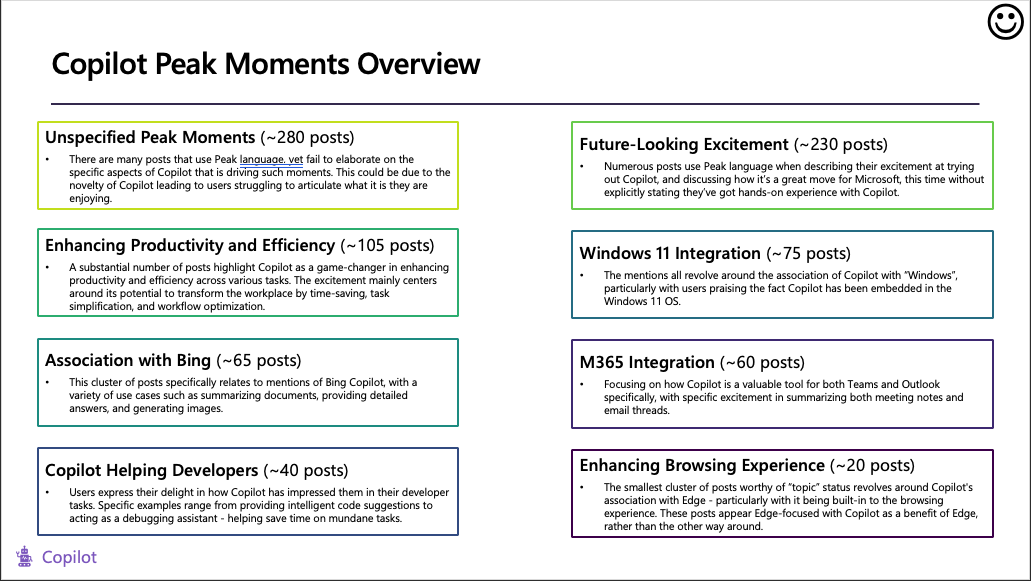
\includegraphics{img/peaks_list.png}

}

\caption{Screenshot from a Peaks and Pits project showcasing the
identified Peak moments for a product at a high level}

\end{figure}%

\subsection{Key features of project}\label{key-features-of-project}

\begin{itemize}
\tightlist
\item
  There is no out-of-the-box ML model available whose purpose is to
  classify social media posts as either peaks or pits (i.e.~we cannot
  use a ready-made solution, we must design our own bespoke solution).
\item
  There is limited data available

  \begin{itemize}
  \tightlist
  \item
    Unlike the case of spam/ham or sentiment classification, there is
    not a bank of pre-labelled data available for us to leverage for
    `traditional ML'.
  \end{itemize}
\item
  Despite these issues, the research problem itself is well defined
  (\textbf{what} are the core peak and pit moments for a brand/product),
  and because there are only three classes (peak, pit, or neither) which
  are based on extensive research, the classes themselves are well
  described (even if it is case of ``you know a peak moment when you see
  it'').
\end{itemize}

\section{Overview of approach}\label{overview-of-approach}

Peaks and pits projects have gone through many iterations throughout the
past year and a half. Currently, the general workflow is to use utilise
a model framework known as
\href{https://huggingface.co/docs/setfit/conceptual_guides/setfit}{SetFit}
to efficiently train a text classification model with limited training
data. This fine-tuned model is then able to run inference over large
datasets to label posts as either peaks, pits, or neither. We then
utilise the LLM capabilities to refine these peak and pit moments into a
collection of posts we are extremely confident are peaks and/or pits. We
then employ topic modelling to identify groups of similar peaks and pits
to help us organise and discover hidden topics or themes within this
collection of core moments.

This whole process can be split into six distinct steps:

\begin{enumerate}
\def\labelenumi{\arabic{enumi}.}
\tightlist
\item
  \hyperref[step-one]{Extract brand/product mentions from Sprinklr (the
  start of any project)}
\item
  \hyperref[step-two]{Obtain project-specific exemplar posts to help
  fine-tune a text classification model}
\item
  \hyperref[step-three]{Perform model fine-tuning through contrastive
  learning}
\item
  \hyperref[step-four]{Run inference over all of the project specific
  data}
\item
  \hyperref[step-five]{Use GPT-3.5 for an extra layer of classification
  on identified peaks and pits}
\item
  \hyperref[step-six]{Turn moments into something interpretable using
  topic modelling}
\end{enumerate}

\begin{figure}[H]

{\centering 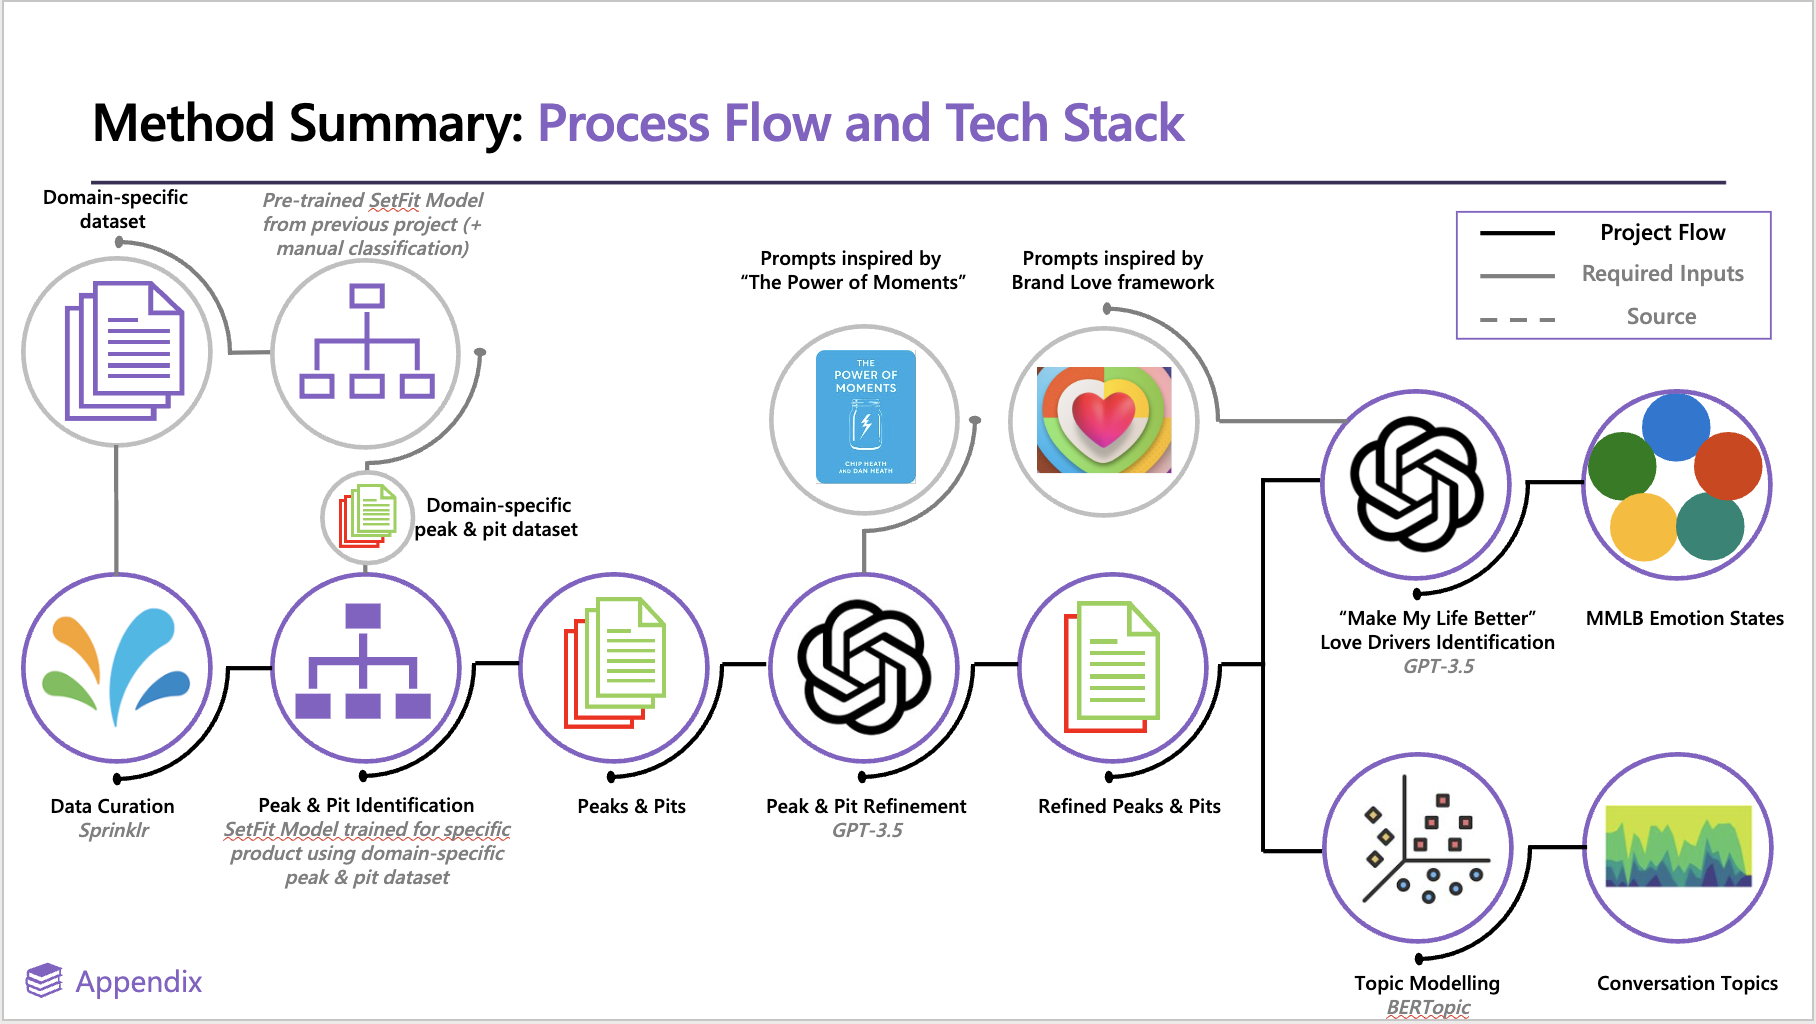
\includegraphics[width=0.8\textwidth,height=\textheight]{./img/ar_workflow.png}

}

\caption{Schematic workflow from Project 706 - Peaks and Pits in M365
Apps}

\end{figure}%

\subsection{Obtain posts for the project (Step 1)}\label{step-one}

This step relies on the analysts to export relevant mentions from
Sprinklr (one of the social listening tools that analysts utilise to
obtain social data), and therefore is not detailed much here. What is
required is one dataset for each of the brands/products, so they can be
analysed separately.

\subsection{Identify project-specific exemplar peaks and pits to
fine-tune our ML model (Step 2)}\label{step-two}

This step is synonymous with data labelling required for any machine
learning project where annotated data is not already available.

Whilst there is no one-size-fits-all for determining the amount of data
required to train a machine learning model, for traditional models and
tasks, the number of examples per label is often in the region of
thousands, and often this isn't even enough for more complex problems.

The time required to accurately label thousands of peaks and pits to
train a classification model in the traditional way is sadly beyond the
scope of feasibility for our projects. As such we needed an approach
that did not rely on copious amounts of pre-labelled data.

This is where
\href{https://huggingface.co/docs/setfit/conceptual_guides/setfit}{SetFit}
comes in. As mentioned previously, SetFit is a framework that enables us
to efficiently train a text classification model with limited training
data.

\begin{tcolorbox}[enhanced jigsaw, breakable, toprule=.15mm, titlerule=0mm, leftrule=.75mm, opacityback=0, opacitybacktitle=0.6, colbacktitle=quarto-callout-tip-color!10!white, colback=white, bottomrule=.15mm, title=\textcolor{quarto-callout-tip-color}{\faLightbulb}\hspace{0.5em}{How does it do this?}, coltitle=black, colframe=quarto-callout-tip-color-frame, bottomtitle=1mm, toptitle=1mm, arc=.35mm, rightrule=.15mm, left=2mm]

\emph{Note the below is directly copied from the SetFit documentation.
It is so succinctly written that trying to rewrite it would not do it
justice.}

Every SetFit model consists of two parts: a \textbf{sentence
transformer} embedding model (the body) and a \textbf{classifier} (the
head). These two parts are trained in two separate phases: the
\textbf{embedding finetuning phase} and the \textbf{classifier training
phase}. This conceptual guide will elaborate on the intuition between
these phases, and why SetFit works so well.

Embedding finetuning phase The first phase has one primary goal:
finetune a sentence transformer embedding model to produce useful
embeddings for our classification task. The Hugging Face Hub already has
thousands of sentence transformer available, many of which have been
trained to very accurately group the embeddings of texts with similar
semantic meaning.

However, models that are good at Semantic Textual Similarity (STS) are
not necessarily immediately good at our classification task. For
example, according to an embedding model, the sentence of 1)
``\texttt{He\ biked\ to\ work.}'' will be much more similar to 2)
``\texttt{He\ drove\ his\ car\ to\ work.}'' than to 3)
``\texttt{Peter\ decided\ to\ take\ the\ bicycle\ to\ the\ beach\ party!}''.
But if our classification task involves classifying texts into
transportation modes, then we want our embedding model to place
sentences 1 and 3 closely together, and 2 further away.

To do so, we can finetune the chosen sentence transformer embedding
model. The goal here is to nudge the model to use its pretrained
knowledge in a different way that better aligns with our classification
task, rather than making the completely forget what it has learned.

For finetuning, SetFit uses \textbf{contrastive learning}. This training
approach involves creating \textbf{positive and negative pairs} of
sentences. A sentence pair will be positive if both of the sentences are
of the same class, and negative otherwise. For example, in the case of
binary ``positive''-``negative'' sentiment analysis,
(``\texttt{The\ movie\ was\ awesome}'', ``\texttt{I\ loved\ it}'') is a
positive pair, and (``\texttt{The\ movie\ was\ awesome}'',
``\texttt{It\ was\ quite\ disappointing}'') is a negative pair.

During training, the embedding model receives these pairs, and will
convert the sentences to embeddings. If the pair is positive, then it
will pull on the model weights such that the text embeddings will be
more similar, and vice versa for a negative pair. Through this approach,
sentences with the same label will be embedded more similarly, and
sentences with different labels less similarly.

Conveniently, this contrastive learning works with pairs rather than
individual samples, and we can create plenty of unique pairs from just a
few samples. For example, given 8 positive sentences and 8 negative
sentences, we can create 28 positive pairs and 64 negative pairs for 92
unique training pairs. This grows exponentially to the number of
sentences and classes, and that is why SetFit can train with just a few
examples and still correctly finetune the sentence transformer embedding
model. However, we should still be wary of overfitting.

Classifier training phase Once the sentence transformer embedding model
has been finetuned for our task at hand, we can start training the
classifier. This phase has one primary goal: create a good mapping from
the sentence transformer embeddings to the classes.

Unlike with the first phase, training the classifier is done from
scratch and using the labelled samples directly, rather than using
pairs. By default, the classifier is a simple \textbf{logistic
regression} classifier from scikit-learn. First, all training sentences
are fed through the now-finetuned sentence transformer embedding model,
and then the sentence embeddings and labels are used to fit the logistic
regression classifier. The result is a strong and efficient classifier.

Using these two parts, SetFit models are efficient, performant and easy
to train, even on CPU-only devices.

\end{tcolorbox}

There is no perfect number of labelled examples to find per class
(i.e.~peak, pit, or neither). Whilst in general more exemplars (and
hence more training data) is beneficial, having fewer but high quality
labelled posts is far superior than more posts of poorer quality. This
is extremely important due to the contrastive nature of SetFit where
it's superpower is making the most of few, extremely good, labelled
data.

Okay so now we know why we need labelled data, and we know what the
model will do with it, \emph{what is our approach} for obtaining the
labelled data?

Broadly, we use our human judgement to read a post from the current
project dataset, and manually label whether we think it is a peak, a
pit, or neither. To avoid us just blindly reading through random posts
in the dataset in the hope of finding good examples (this is not a good
use of time), we can employ a couple of tricks to narrow our search
region to posts that have a reasonable likelihood of being suitable
examples.

\begin{enumerate}
\def\labelenumi{\arabic{enumi})}
\item
  The first trick is to use the OpenAI API to access a GPT model. This
  involves taking a sample of posts (say \textasciitilde1000) and
  running these through a GPT model, with a prompt that asks the model
  to classify each post into either a peak, pit, or neither. This is
  possible because GPT models have learned knowledge of peaks and pits
  from its training on large datasets. We can therefore get a human to
  only sense-check/label posts that GPT also believes are peaks or pits.
\item
  The second trick involves using a previously created SetFit model
  (i.e.~from an older project), and running inference over a similar
  sample of posts (again, say \textasciitilde1000).
\end{enumerate}

We would tend to suggest the OpenAI route, as it is simpler to implement
(in our opinion), and often the old SetFit model has been finetuned on
data from a different domain so it might struggle to understand domain
specific language in the current dataset. However, be aware if it not as
scalable as using an old SetFit model and has the drawback of being a
prompt based classification of a black-box model (as well as issues
relating to cost and API stability).

Irrespective of which approach is taken, by the end of this step we need
to have a list of example posts we are confident represent what a peak
or pit moment looks like for each particular product we are researching,
including posts that are ``neither''.

\begin{tcolorbox}[enhanced jigsaw, breakable, toprule=.15mm, titlerule=0mm, leftrule=.75mm, opacityback=0, opacitybacktitle=0.6, colbacktitle=quarto-callout-note-color!10!white, colback=white, bottomrule=.15mm, title=\textcolor{quarto-callout-note-color}{\faInfo}\hspace{0.5em}{Why do we do this for each project?}, coltitle=black, colframe=quarto-callout-note-color-frame, bottomtitle=1mm, toptitle=1mm, arc=.35mm, rightrule=.15mm, left=2mm]

After so many projects now don't we already have a good idea of what a
peak and pit moment for the purposes of model training?

Each peak and pit project we work on has the potential to introduce
`domain' specific language, which a machine learning classifier (model)
may not have seen before. By manually identifying exemplar peaks and
pits that are project-specific, this gives our model the best chance to
identify emotional moments appropriate to the project/data at hand.

The obvious case for this is with gaming specific language, where terms
that don't necessarily relate to an `obvious' peak or pit moment could
refer to one the gaming conversation, for example the terms/phrases
``GG'', ``camping'', ``scrub'', and ``goat'' all have very specific
meanings in this domain that differ from their use in everyday language.

\end{tcolorbox}

\subsection{Train our model using our labelled examples (Step
3)}\label{step-three}

Before we begin training our SetFit model with our data, it's necessary
to clean and wrangle the fine-tuning datasets. Specifically, we need to
mask any mentions of brands or products to prevent bias. For instance,
if a certain brand frequently appears in the training data within peak
contexts, the model could erroneously link peak moments to that brand
rather than learning the peak-language expressed in the text.

\begin{quote}
This precaution should extend to all aspects of our training data that
might introduce biases. For example, as we now have examples from
various projects, an overrepresentation of data from `gaming projects'
in our `peak' posts within our training set (as opposed to the `pit'
posts) could skew the model into associating gaming-related language
more with peaks than pits.
\end{quote}

Broadly the cleaning steps that should be applied to our data for
finetuning are:

\begin{itemize}
\tightlist
\item
  Mask brand/product mentions
\item
  Remove hashtags \#️⃣
\item
  Remove mentions 💬
\item
  Remove URLs 🌐
\item
  Remove emojis 🐙
\end{itemize}

\begin{tcolorbox}[enhanced jigsaw, breakable, toprule=.15mm, titlerule=0mm, leftrule=.75mm, opacityback=0, opacitybacktitle=0.6, colbacktitle=quarto-callout-note-color!10!white, colback=white, bottomrule=.15mm, title=\textcolor{quarto-callout-note-color}{\faInfo}\hspace{0.5em}{What about other cleaning steps?}, coltitle=black, colframe=quarto-callout-note-color-frame, bottomtitle=1mm, toptitle=1mm, arc=.35mm, rightrule=.15mm, left=2mm]

You will notice here we do not remove stop words-. As explained in the
previous step, part of the finetuning process is to finetune a sentence
embedding model, and we want to keep stop words so that we can use the
full context of the post in order to finetune accurate embeddings.

\end{tcolorbox}

At this step, we can split out our data into training, testing, and
validation datasets. A good rule of thumb is to split the data 70\% to
training data, 15\% to testing data, and 15\% to validation data. By
default,
\href{https://huggingface.co/docs/setfit/v1.0.3/en/conceptual_guides/sampling_strategies}{SetFit
oversamples} the minimum class within the training data, so we
\emph{shouldn't} have to worry too much about imbalanced datasets-
though be aware if we have extreme imbalanced we will end up sampling
the same contrastive pairs (normally positive pairs) multiple times.
However, our experimentation has shown that class imbalance doesn't seem
to have a significant effect to the training/output of the SetFit model
for peaks and pits.

We are now at the stage where we can actually fine-tune the model. There
are many different parameters we can change when fine-tuning the model,
such as the specific embedding model used, the number of epochs to train
for, the number of contrastive pairs of sentences to train on etc. For
more details, please refer to the
\href{https://jamiehshare.github.io/peaks-pits-bookdown/step-four.html}{Peaks
and Pits Playbook}

We can assess model performance on the testing dataset by looking at
accuracy, precision, recall, and F1 scores. For peaks and pits, the most
important metric is actually \textbf{recall} because in
\hyperref[step-four]{step 4} we reclassify posts using GPT, so we want
to make sure we are able to provide \emph{as many true peak/pit moments
as possible} to this step, even if it means we also provide a few false
positives.

\begin{tcolorbox}[enhanced jigsaw, breakable, toprule=.15mm, titlerule=0mm, leftrule=.75mm, opacityback=0, opacitybacktitle=0.6, colbacktitle=quarto-callout-note-color!10!white, colback=white, bottomrule=.15mm, title=\textcolor{quarto-callout-note-color}{\faInfo}\hspace{0.5em}{Click here for more info as to why recall is most important}, coltitle=black, colframe=quarto-callout-note-color-frame, bottomtitle=1mm, toptitle=1mm, arc=.35mm, rightrule=.15mm, left=2mm]

As a refresher, \texttt{precision} is the \emph{proportion of positive
identifications} that are actually \emph{correct} (it focuses on the
correctness of positive predictions) whereas \texttt{recall} is the
\emph{proportion of actual positives} that are identified correctly (it
focuses on capturing all relevant instances).

In cases where false positives need to be minimised (incorrectly
predicting a non-event as an event) we need to prioritise
\texttt{precision} - if you've built a model to identify hot dogs from
regular ol' doggos, high precision ensures that normal dogs are not
misclassified as hot dogs.

In cases where false negatives need to be minimised (failing to detect
an actual event) we need to prioritise \texttt{recall} - in medical
diagnoses we need to minimise the number of times a patient is
incorrectly told they \emph{do not} have a disease when in reality they
\emph{do} (or worded differently, we need to ensure that
\textbf{\emph{all}} patients with a disease are identified).

To apply this to our problem- we want to be sure that we capture all (or
as many as possible) relevant instances of peaks or pits- even if a few
false positives come in (neither posts that are incorrectly classified
as peaks or pits). As we use GPT to make further peak/pit
identifications, it's better to provide GPT with with a comprehensive
set of potential peaks and pits, including some incorrect ones, than to
miss out on critical data.

\end{tcolorbox}

\subsubsection*{Visualise model
separation}\label{visualise-model-separation}
\addcontentsline{toc}{subsubsection}{Visualise model separation}

As a bonus, we can actually neatly visualise how well our finetuning of
the sentence transformer embedding model has gone- by seeing how well
the model is able to separate our different classes in embedding space.

We can do this by visualising the 2-D structure of the embeddings and
see how they cluster:

This is what it looks the embeddings space looks like on an un-finetuned
model:

\begin{figure}[H]

{\centering 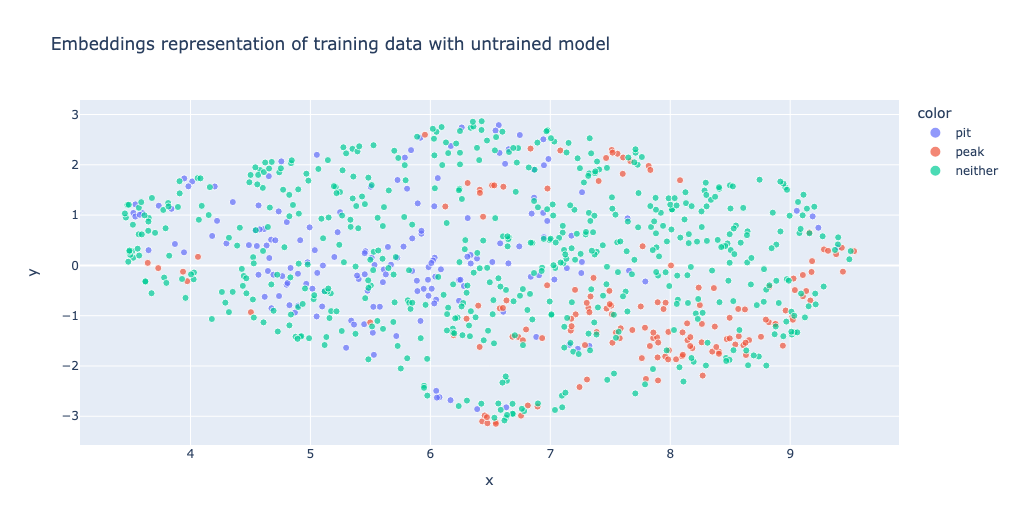
\includegraphics{./img/embedding_untrained.png}

}

\caption{Un-finetuned embedding model}

\end{figure}%

Here we can see that posts we know are peaks, pits, and neither all
overlap and there is no real structure in the data. Any clustering of
points observed are probably due to the posts' semantic similarity (c.f.
the mode of transport example above). We would not be able to nicely use
a classifier model to get a good mapping from this embedding space to
our classes (i.e.~we couldn't easily separate classes here).

By visualising the same posts after finetuning the embedding model, we
get something more like this, where we can see that the embedding model
now clearly separates posts based on their peak/pit classification
(though we must be wary of overfitting!).

\begin{figure}[H]

{\centering 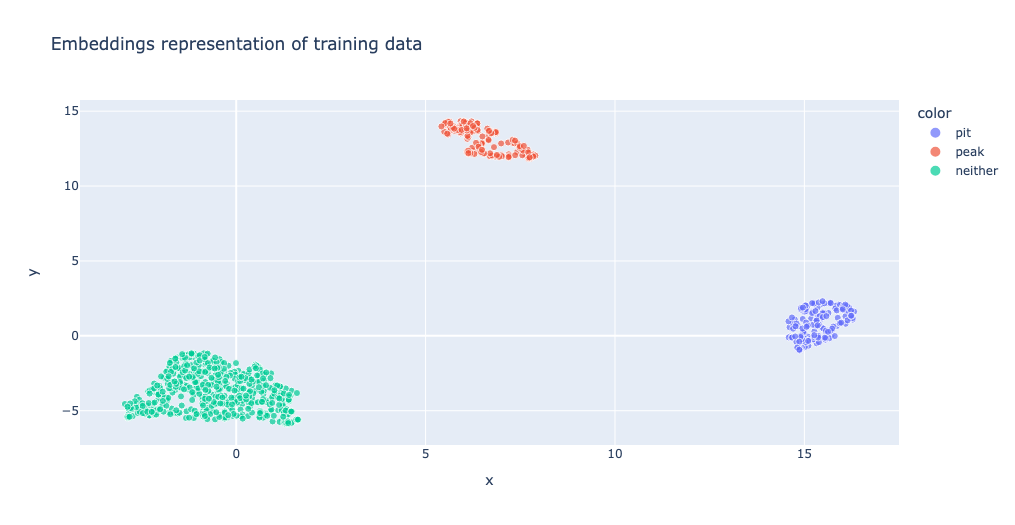
\includegraphics{./img/embedding_trained.png}

}

\caption{Finetuned embedding model}

\end{figure}%

Finally, now we are happy with our model performance based on the
training and validation datasets, we can evaluate the performance of
this final model using our testing data. This is data that the model has
never seen, and we are hoping that the accuracy and performance is
similar to that of the validation data. This is Machine Learning 101 and
if a refresher is needed for this there are plenty of resources online
looking at the role of training, validation, and testing data.

\subsection{Run inference over project data (Step 4)}\label{step-four}

It is finally time to infer whether the project data contain peaks or
pits by using our fine-tuned SetFit model to classify the posts.

Before doing this again we need to make sure we do some data cleaning on
the project specific data.

Broadly, this needs to match the high-level cleaning we did during
fine-tuning stage:

\begin{itemize}
\tightlist
\item
  Mask brand/product mentions (using RoBERTa-based model {[}or
  similar{]} and \texttt{Rivendell} functions)
\item
  Remove hashtags \#️⃣
\item
  Remove mentions 💬
\item
  Remove URLs 🌐
\item
  Remove emojis 🐙
\end{itemize}

\begin{tcolorbox}[enhanced jigsaw, breakable, toprule=.15mm, titlerule=0mm, leftrule=.75mm, opacityback=0, opacitybacktitle=0.6, colbacktitle=quarto-callout-warning-color!10!white, colback=white, bottomrule=.15mm, title=\textcolor{quarto-callout-warning-color}{\faExclamationTriangle}\hspace{0.5em}{Note on social media sources}, coltitle=black, colframe=quarto-callout-warning-color-frame, bottomtitle=1mm, toptitle=1mm, arc=.35mm, rightrule=.15mm, left=2mm]

Currently all peak and pit projects have been done on Twitter or Reddit
data, but if a project includes web/forum data quirky special
characters, numbered usernames, structured quotes etc. should also be
removed.

\end{tcolorbox}

Okay now we can \emph{finally} run inference. This is extremely simple
and only requires a couple of lines of code (again see the
\href{https://jamiehshare.github.io/peaks-pits-bookdown/step-five.html}{Peaks
and Pits Playbook for code implementation})

\subsection{The metal detector, GPT-3.5 (Step 5)}\label{step-five}

During \hyperref[step-four]{step 4} we obtained peak and pit
classification using few-shot classification with SetFit. The benefit of
this approach (as outlined previously) is its speed and ability to
classify with very few labelled samples due to contrastive learning.

However, during our iterations of peak and pit projects, we've realised
that this step still classifies a fair amount of non-peak and pit posts
incorrectly. This can cause noise in the downstream analyses and be very
time consuming for us to further trudge through verbatims.

As such, the aim of this step is to further our confidence in our final
list of peaks and pits to be \emph{actually} peaks and pits. Remember
before we explained that for SetFit, we focussed on \textbf{recall}
being the most important measure in our business case? This is where we
assume that GPT-3.5 enables us to remove the false positives due to it's
incredibly high performance.

\begin{tcolorbox}[enhanced jigsaw, breakable, toprule=.15mm, titlerule=0mm, leftrule=.75mm, opacityback=0, opacitybacktitle=0.6, colbacktitle=quarto-callout-important-color!10!white, colback=white, bottomrule=.15mm, title=\textcolor{quarto-callout-important-color}{\faExclamation}\hspace{0.5em}{Why not use GPT from the start?}, coltitle=black, colframe=quarto-callout-important-color-frame, bottomtitle=1mm, toptitle=1mm, arc=.35mm, rightrule=.15mm, left=2mm]

Using GPT-3.5 for inference, even over relatively few posts as in peaks
and pits, is expensive both in terms of time and money. Preliminary
tests have suggested it is in the order of magnitude of thousands of
times slower than SetFit. It is for these reasons why we do not use
GPT-x models from the get go, despite it's obvious incredible
understanding of natural language.

\end{tcolorbox}

Whilst prompt-based classification such as those with GPT-3.5 certainly
has its drawbacks (dependency on prompt quality, prompt injections in
posts, handling and version control of complex prompts, unexpected
updates to the model weights rendering prompts ineffective), the
benefits include increased flexibility in what we can ask the model to
do. As such, in the absence of an accurate, cheap, and quick model to
perform span detection, we have found that often posts identified as
peaks/pits did indeed use peak/pit language, but the context of the
moment was not related to the brand/product at the core of the research
project.

For example, take the post that we identified in the project 706,
looking for peaks and pits relating to PowerPoint:

\begin{quote}
This brings me so much happiness! Being a non-binary graduate student in
STEM academia can be challenging at times. Despite using my they/them
pronouns during introductions, emails, powerpoint presentations, name
tags, etc. my identity is continuously mistaken. Community is key!
\end{quote}

This is clearly a `peak', however it is not accurate or valid to
attribute this memorable moment to PowerPoint. Indeed, PowerPoint is
merely mentioned in the post, but is not a core driver of the Peak which
relates to feeling connection and being part of a community. This is as
much a PowerPoint Peak as it is a Peak for the use of emails.

Therefore, we can engineer our prompt to include a caveat to say that
the specific peak or pit moment must relate directly to the
brand/product usage (if relevant).

\subsection{Topic modelling to make sense of our data (Step
6)}\label{step-six}

Now we have an extremely refined set of posts classified as either peak
or pits. The next step is to identify what these moments actually relate
to (i.e.~identify the topics of these moments through statistical
methods).

To do this, we employ topic modelling via
\href{https://maartengr.github.io/BERTopic/index.html}{BERTopic} to
identifying high-level topics that emerge within the peak and pit
conversation. This is done separately for each product and peak/pit
dataset (i.e.~there will be one BERTopic model for product A peaks,
another BERTopic model for product A pits, an additional BERTopic model
for product B peaks etc).

We implement BERTopic using the R package BertopicR. As there is already
\href{https://aoiferyan-sc.github.io/BertopicR/}{good documentation on
BertopicR} this section will not go into any technical detail in regards
to implementation.

From BertopicR. we end up with a topic label for each post in our
dataset, meaning we can easily quantify the size of each topics and
visualise temporal patterns of topic volume etc.

\bookmarksetup{startatroot}

\chapter{AI landscape}\label{ai-landscape}

Timbo use this qmd to write everything you need for the AI landscape.

\subsection{Background of project}\label{background-of-project}

Explain here why Microsoft wanted to perform the project, and the
overall goal of the project.

\subsection{Final output of project}\label{final-output-of-project}

Couple of images of the landscape perhaps- with a summary outlining what
was found (don't worry about specific project details, something like
``distinct topics of conversation found by human interpretation of the
landscape'' is better than ``in 726 we found 15 new topics of which
conversational AI evolved to encompass the ethics topic'' which is too
specific)

\subsection{How to get there}\label{how-to-get-there}

Go through a step by step approach as to how one would go about the
project. For now, again don't worry about details (etc I wouldn't worry
about the particular embedding model here, just say that the posts were
embedded using a sentence transformer model etc).

Feel free to add screenshots of things where needed

\bookmarksetup{startatroot}

\chapter{Summary}\label{summary}

In summary, this book has no content whatsoever.

\begin{Shaded}
\begin{Highlighting}[]
\DecValTok{1} \SpecialCharTok{+} \DecValTok{1}
\end{Highlighting}
\end{Shaded}

\begin{verbatim}
[1] 2
\end{verbatim}

\bookmarksetup{startatroot}

\chapter*{References}\label{references}
\addcontentsline{toc}{chapter}{References}

\markboth{References}{References}

\phantomsection\label{refs}
\begin{CSLReferences}{0}{1}
\end{CSLReferences}



\end{document}
